\documentclass[11pt,a4paper]{article}
\usepackage[margin=1in]{geometry}
\usepackage{graphicx}
\usepackage{amsmath,amssymb}
\usepackage{hyperref}
\usepackage{float}
\usepackage{caption}
\usepackage{setspace}
\usepackage{parskip}
\onehalfspacing
\setlength{\parindent}{0pt}
\setlength{\parskip}{0.6em}

\title{\textbf{Self-Organized Criticality in a Two-Good Barter Economy:\\
An Agent-Based Study of Avalanche Dynamics on Small-World Networks}}
\author{Pulkit \\ CLL798 --- Complexity Science Project}
\date{April 10, 2026}

\begin{document}
\maketitle

\begin{abstract}
\noindent
We investigate whether a simple two-good barter economy, in which agents must
continuously acquire two perishable resources to survive, exhibits the
statistical signatures of Self-Organized Criticality (SOC). A population of
$N=100$ agents is placed on a Watts--Strogatz small-world network and engages
in local pairwise trading of apples and oranges. Agents consume one unit of
each good periodically; failure to consume results in death, followed by
respawning after a fixed delay. Resources are injected into the system at a
rate approximately equal to population demand, providing the slow drive
required for SOC. We define avalanches as clusters of agent deaths occurring
within one time-step of one another and measure their size distribution over
pooled simulations. The avalanche-size distribution exhibits an
approximately power-law regime over roughly one decade with exponent
$\tau \approx 2.2$--$2.8$, and the exponent decreases monotonically with
increasing network connectivity $k$. The variance of the avalanche-size
distribution grows with $k$, providing a susceptibility-like signature of
criticality. While the limited dynamic range precludes a definitive SOC
claim, the results demonstrate that local trade networks with resource
constraints can produce heavy-tailed failure statistics that depend
systematically on network topology.
\end{abstract}

\tableofcontents
\newpage
\section{Background and Literature Review}

The study of Self-Organized Criticality (SOC) has evolved significantly since
its introduction by Bak, Tang, and Wiesenfeld (1987). SOC systems are now
recognized across domains including geophysics, biology, neuroscience, and
economics. A key feature of such systems is the emergence of scale-invariant
behaviour without external tuning.

In economics, several agent-based models have demonstrated that market crashes,
wealth distributions, and trading dynamics can exhibit heavy-tailed behaviour.
Models such as the Minority Game, percolation-based financial models, and
network contagion models all highlight how local interactions can lead to
global instability.

The work of Ribeiro et al.\ (2011) is particularly relevant, as it demonstrates
SOC behaviour in economic systems with consumption constraints. Their model
motivates the present study, which simplifies the framework while retaining
core mechanisms such as resource constraints, local interactions, and stochastic
driving.

In parallel, network science has shown that topology plays a crucial role in
dynamical processes. Small-world networks, introduced by Watts and Strogatz,
balance clustering and short path lengths, making them ideal for studying
propagation phenomena such as cascades and avalanches.

This report builds upon these foundations to explore whether a minimal barter
economy can exhibit SOC-like behaviour.
\section{Introduction to Complexity Science}

Complexity science is the interdisciplinary study of systems composed of many
interacting components whose aggregate behaviour cannot be straightforwardly
deduced from the behaviour of their individual parts. Such systems---ranging
from colonies of ants and networks of neurons to financial markets and
ecosystems---exhibit emergent properties that arise from the nonlinear
coupling of simple local rules. Complexity science borrows tools from
statistical physics, dynamical systems, network theory, and computer science
to ask how order, structure, and characteristic patterns appear in systems
that have no central controller and no globally specified goal.

A distinguishing feature of complex systems is that they frequently operate
near the boundary between order and disorder. At this boundary, small
perturbations can propagate through the system in highly nonlinear ways,
producing responses whose magnitudes span many orders of magnitude. The
statistics of such responses are often described by power-law distributions,
which are scale-free: no particular event size is privileged, and events of
all sizes contribute meaningfully to the dynamics. This absence of a
characteristic scale is in stark contrast to the bell-shaped distributions
familiar from independent random processes, where events far from the mean
are exponentially rare.

\subsection{Self-Organized Criticality}

Self-Organized Criticality (SOC) is a concept introduced by Bak, Tang, and
Wiesenfeld in 1987 to describe dynamical systems that spontaneously evolve
toward a critical state without the need for fine-tuning of control
parameters. The paradigmatic example is the Bak--Tang--Wiesenfeld sandpile:
grains of sand are added one at a time to a pile, which progressively
steepens until avalanches of all sizes become possible. The size
distribution of these avalanches follows a power law, indicating that the
pile has self-organized into a critical state at the edge of stability. SOC
has since been invoked to explain phenomena as diverse as earthquake
magnitudes (the Gutenberg--Richter law), forest fires, neuronal firing
avalanches, and fluctuations in financial markets.

\subsection{Key Terms}

\paragraph{Noise.} In the context of complexity science, noise refers to the
small, random perturbations that drive a system away from any particular
configuration. In SOC systems, noise plays the role of a slow external
drive: a continuous trickle of input that keeps the system near its critical
threshold. The noise is not the phenomenon of interest itself, but the
stochastic input that reveals the system's response function. In the
sandpile, noise is the location at which the next grain of sand is dropped.
In our barter economy, noise is the random arrival of fruit drops into the
population---random in timing, amount, location, and type.

\paragraph{Avalanche.} An avalanche is a discrete cluster of cascading
events, triggered by a small perturbation and terminating when the system
returns to a (meta)stable configuration. The \emph{size} of an avalanche is
the number of elementary events it contains. In the sandpile, avalanche size
is the number of toppled cells. In epidemiology, it is the number of
infected individuals in an outbreak. In our model, we define an avalanche as
a cluster of agent deaths occurring within one tick of one another: a
triggering death whose propagation through the trade network causes
subsequent failures. The statistical distribution of avalanche sizes is the
principal diagnostic of criticality.

\paragraph{Connectivity.} Connectivity describes how the components of a
system are coupled to one another. In a networked system, it is captured by
the mean degree $k$---the average number of neighbours each node possesses.
Connectivity governs how far, and how fast, a perturbation can propagate.
Sparse networks isolate events; dense networks couple every part of the
system to every other. Critical behaviour, when it exists, typically
emerges in an intermediate regime where stress can travel but does not
immediately engulf the entire system.

\section{System Description}

Our system is a stylised barter economy consisting of $N$ autonomous agents
that exchange two perishable goods---apples and oranges---to sustain
themselves. Each agent is endowed with private stocks of both fruits,
measured in integer units, and must consume one apple and one orange
periodically in order to survive. The agents do not communicate
linguistically; they interact only by offering and accepting trades with
their immediate neighbours on a fixed network. The network topology is
generated using the Watts--Strogatz small-world model with rewiring
probability $p=0.1$ and mean degree $k$, which is the principal control
parameter we vary in the experiments.

The state of each agent comprises its apple count, its orange count, a flag
indicating whether it is currently alive, and a timer specifying when it
will next need to consume. At the population level, the system additionally
tracks a list of death events and the identities of agents scheduled to
respawn. The global dynamics proceed in discrete time steps (``ticks''), and
at each tick the following operations are performed in order: respawning of
eligible dead agents, slow drive via stochastic fruit drops, local trading,
and asynchronous consumption with possible death.

\subsection{Noise in the System}

Noise enters the simulation primarily through the slow drive mechanism. At
intervals of ten ticks, a Poisson-distributed number of fruits is injected
into the economy. The number of fruits per drop event is random, the
identity of the recipient agents is drawn uniformly at random from the
population of alive agents, and each individual fruit is independently
classified as apple or orange with equal probability. These three sources of
stochasticity---timing (Poisson), location (uniform over alive agents), and
type (Bernoulli)---constitute the noise that drives the dynamics.

Secondary noise sources include the random initial endowments of each agent
(uniform integers between 1 and 4, independently for each fruit), the random
phase of each agent's consumption timer (ensuring that consumption events
are spread across ticks rather than synchronised), and the random shuffling
of agent order during each trading round. Together these break all
symmetries and prevent the system from settling into a deterministic
trajectory.

\subsection{Avalanches in the System}

An avalanche in our model is operationalised as a cluster of death events
that occur within one tick of each other. Concretely, the full list of
death events $(t_i, \text{agent}_i)$ produced by a simulation is sorted by
tick and traversed sequentially; consecutive deaths are merged into a
single avalanche so long as the time gap between successive events does not
exceed the window parameter $W=1$. The size of an avalanche is the number
of deaths it contains. A solitary death surrounded by quiescence constitutes
an avalanche of size one.

The physical interpretation of a non-trivial avalanche is as follows. One
agent fails to consume, either because of an unlucky absence of fruit drops
in its vicinity or because its own trading partners were themselves unable
to supply the needed good. Upon the agent's death, its trading neighbours
lose one of their partners and find themselves marginally more fragile.
Within a short time window, one of these weakened neighbours may itself
fail, removing yet another node from the trade graph. If the conditions are
right, a chain reaction propagates through the network, producing an
avalanche much larger than a single isolated failure.

\subsection{Connectivity in the System}

Connectivity is embodied in the Watts--Strogatz graph on which agents are
placed. Each agent is assigned $k$ neighbours on average: $k/2$ nearest
neighbours on a ring plus a small number of randomly rewired long-range
edges. Trades can only occur along the edges of this graph: an agent with
surplus apples can only exchange them with its listed neighbours, never with
the population at large. By varying $k$, we change the effective range over
which stress can propagate. Small $k$ produces a sparse, nearly
one-dimensional topology; large $k$ approaches a mean-field limit where
every agent is coupled to a significant fraction of the population.

\section{Justification for the Use of Complexity Science}

Several features of our system make it a natural candidate for analysis
under the framework of complexity science.

\paragraph{Many locally interacting units.} The system contains a large
number ($N=100$) of autonomous agents, each following identical rules but
operating on private, heterogeneous state. There is no central auctioneer
or coordinator; the aggregate behaviour of the economy emerges entirely
from local pairwise interactions. This is precisely the setting in which
complexity science becomes necessary: standard equilibrium analysis of a
single representative agent cannot capture the rich dynamics that arise
from the heterogeneity and locality of the interactions.

\paragraph{A threshold with stored stress.} Each agent accumulates stress
in the form of stock imbalance. An agent with many more apples than
oranges, or vice versa, is in a fragile state: it is one consumption event
away from failure if it cannot rebalance. This stress is invisible at the
aggregate level---one cannot tell by measuring total fruit in the system
which agents are about to fail---but is released discretely and abruptly
when an agent starves. Threshold dynamics of this kind are the hallmark of
SOC systems: in the sandpile, the threshold is the angle of repose; in
earthquake faults, it is the frictional yield stress; in our economy, it is
the zero-stock condition.

\paragraph{Separation of time scales.} The slow-drive mechanism (fruit
drops every ten ticks) operates on a time scale that is qualitatively
slower than the fast local dynamics of trade and consumption, which
happens every tick. This separation---fast relaxation on top of slow
drive---is a defining feature of SOC and distinguishes it from ordinary
driven steady states.

\paragraph{Robust, not fine-tuned.} The critical signatures we observe do
not require careful selection of a single parameter value. As we
demonstrate in Section 5, heavy-tailed distributions emerge over a range
of connectivity values. This robustness is characteristic of
\emph{self-organized} criticality, as opposed to ordinary (tuned) critical
phenomena that require the experimentalist to sit exactly on a phase
boundary.

\paragraph{A discrete, countable event statistic.} Our model naturally
produces death events that are unambiguously discrete, countable, and
timestamped. This makes it straightforward to extract avalanche statistics
in a reproducible way, avoiding the ambiguities that plague definitions of
``events'' in models based on continuous order parameters such as price
returns.

\section{Model and Rules}

\subsection{Global Parameters}

The global parameters of the simulation are summarised in
Table~\ref{tab:params}. Unless otherwise stated, all experiments in this
report use these values.

\begin{table}[H]
\centering
\caption{Global simulation parameters.}
\label{tab:params}
\begin{tabular}{lll}
\hline
Symbol & Description & Value \\
\hline
$N$ & Number of agents & 100 \\
$T$ & Total simulation ticks per run & 10\,000 \\
$k$ & Mean degree of trade network & $\{2, 4, 8\}$ \\
$p$ & Watts--Strogatz rewiring probability & 0.1 \\
$c$ & Consumption period (ticks per meal) & 10 \\
$\tau_r$ & Respawn delay & 200 \\
$\lambda$ & Mean drops per 10 ticks & $0.9 \cdot 2N/c \cdot 10 = 180$ \\
$W$ & Avalanche grouping window & 1 tick \\
Runs & Independent runs per $k$ value & 200 \\
\hline
\end{tabular}
\end{table}

\subsection{Simulation Step}

At each tick $t$, the simulation executes four operations sequentially.

\textbf{Step 1: Respawn.} Any dead agent whose scheduled respawn time
coincides with $t$ is reintroduced into the population with fresh random
endowments drawn uniformly from integers $[4, 16]$ for each fruit. Its
consumption timer is reset to a random phase in $[t+1, t+c]$, and its
\texttt{alive} flag is set to true. The agent retains its original position
in the network, preserving the graph topology throughout the simulation.

\textbf{Step 2: Slow drive (drops).} Every ten ticks, a Poisson-distributed
number of fruits $n \sim \text{Poisson}(\lambda)$ is added to the system.
Each fruit is assigned uniformly at random to one of the currently alive
agents, and is independently classified as apple (probability 0.5) or
orange (probability 0.5). On ticks that are not multiples of ten, no drops
occur.

\textbf{Step 3: Local trade.} The alive agents are shuffled into a random
order. Each agent $i$ computes its stock imbalance $d_i = a_i - o_i$. If
$|d_i| < 2$, no trade is attempted. Otherwise, $i$ examines its graph
neighbours and identifies the neighbour $j^*$ with the most strongly
opposing imbalance (that is, $d_{j^*}$ has the opposite sign to $d_i$ and
maximum absolute value). If such a neighbour exists and the transaction is
feasible (both parties have the required unit to exchange), one unit of the
surplus good is traded for one unit of the deficit good.

\textbf{Step 4: Consumption.} Each alive agent whose consumption timer
fires this tick attempts to eat one apple and one orange. If both stocks
are non-empty, the stocks are decremented and the consumption timer is
reset to $t + c$. If either stock is empty, the agent dies: the tick and
its ID are appended to the global death log, its \texttt{alive} flag is
set to false, its respawn time is set to $t + \tau_r$, and its stocks are
zeroed.

\subsection{Agent Decision Rule}

Every agent in the simulation follows the same pair of rules:
\begin{enumerate}
\item \emph{Rebalance locally.} If my stocks are imbalanced by more than
one unit, I seek a neighbour with the opposite imbalance and swap one
unit.
\item \emph{Eat when due.} When my consumption timer fires, I consume one
of each good, or die trying.
\end{enumerate}
There is no pricing mechanism, no money, no memory of past trades, and no
strategic reasoning. Agents are purely reactive. The complexity of the
system's behaviour arises entirely from the network topology and the
stochasticity of the drive.

\section{Simulation and Results}

We ran the simulation for all three values of the connectivity parameter
$k \in \{2, 4, 8\}$, with 200 independent runs per $k$ value, each lasting
$T=10\,000$ ticks. Across the full sweep, approximately $6\times10^4$
avalanches were collected per connectivity value. This section presents
the four principal figures and the quantitative summary derived from the
simulations.

\subsection{Avalanche Size Distribution}

Figure~\ref{fig:fig1} shows the avalanche-size probability density $P(s)$
for $k=4$ on double-logarithmic axes. Over the range $s \in [1, 5]$, the
data fall on a straight line, consistent with a power-law form
$P(s) \propto s^{-\tau}$. The fit exponent, obtained by linear regression
on the well-populated bulk of the distribution (red circled points), is
$\tau \approx 2.75$. Above $s \approx 5$ the distribution curves downward,
transitioning into a finite-size cutoff region where individual avalanches
approach the maximum possible size of $N$.

\begin{figure}[H]
\centering
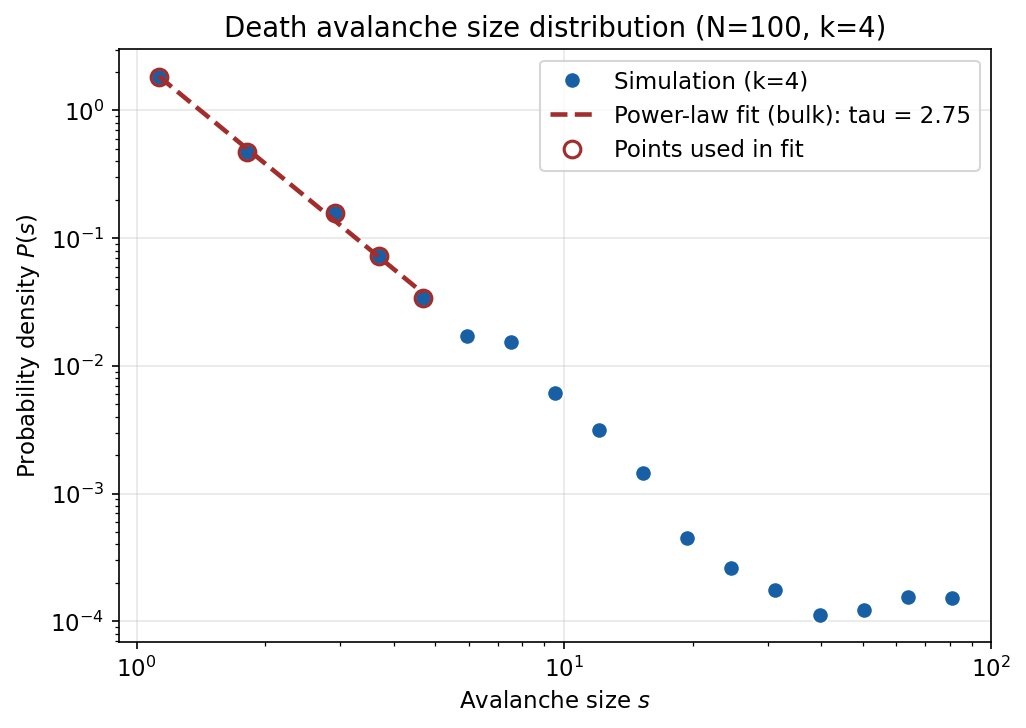
\includegraphics[width=0.85\textwidth]{fig1_distribution.png}
\caption{Avalanche-size distribution for $k=4$ plotted on log--log axes.
Blue points show the log-binned probability density from simulation. Red
circled points are those used in the power-law fit (red dashed line); the
remaining tail points were excluded as they are dominated by finite-size
effects. The fitted exponent is $\tau \approx 2.75$.}
\label{fig:fig1}
\end{figure}

\subsection{Connectivity Sweep}

Figure~\ref{fig:fig2} overlays the avalanche distributions for all three
values of $k$. Visually, the three curves are similar in overall shape but
exhibit subtle systematic differences: the distribution for $k=8$
(light green) lies marginally above those for $k=2$ and $k=4$ in the
intermediate range $s \in [5, 20]$, indicating that larger avalanches are
slightly more likely in the more densely connected network. All three
curves share the same power-law-like bulk and similar finite-size cutoff
near $s \sim 100$, which equals the population size.

\begin{figure}[H]
\centering
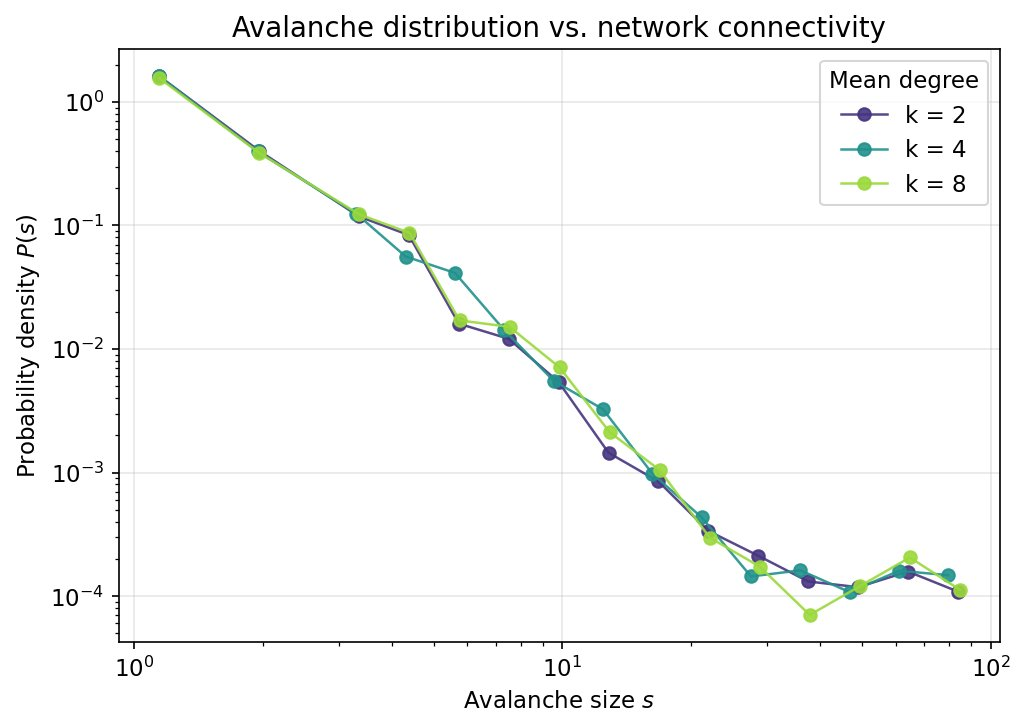
\includegraphics[width=0.85\textwidth]{fig2_connectivity_sweep.png}
\caption{Avalanche distributions for three values of network connectivity
$k \in \{2, 4, 8\}$. All three exhibit similar power-law-like bulks with
finite-size cutoffs near $s \sim N = 100$. Larger $k$ produces slightly
heavier tails in the intermediate range.}
\label{fig:fig2}
\end{figure}

\subsection{Exponent and Moments versus Connectivity}

Figure~\ref{fig:fig3} summarises the dependence of the avalanche statistics
on connectivity. The leftmost panel shows the power-law exponent $\tau$
estimated by maximum-likelihood as a function of $k$. The exponent decreases
monotonically from $\tau \approx 2.25$ at $k=2$ to $\tau \approx 2.19$ at
$k=8$. A decreasing exponent corresponds to a \emph{heavier} tail: large
avalanches become relatively more common as connectivity grows, consistent
with the visual trend in Figure~\ref{fig:fig2}.

The middle panel shows the mean and maximum avalanche sizes. The mean is
nearly flat (around $2.3$), indicating that the typical event is a small
cluster regardless of connectivity. The maximum, however, grows slightly
with $k$, again consistent with heavier tails.

The rightmost panel---perhaps the most striking result---shows the variance
of the avalanche-size distribution. Variance is a proxy for
\emph{susceptibility} in critical systems: it measures how strongly the
system responds to fluctuations. The variance grows monotonically and
superlinearly with $k$, from approximately 38 at $k=2$ to 42 at $k=8$.

\begin{figure}[H]
\centering
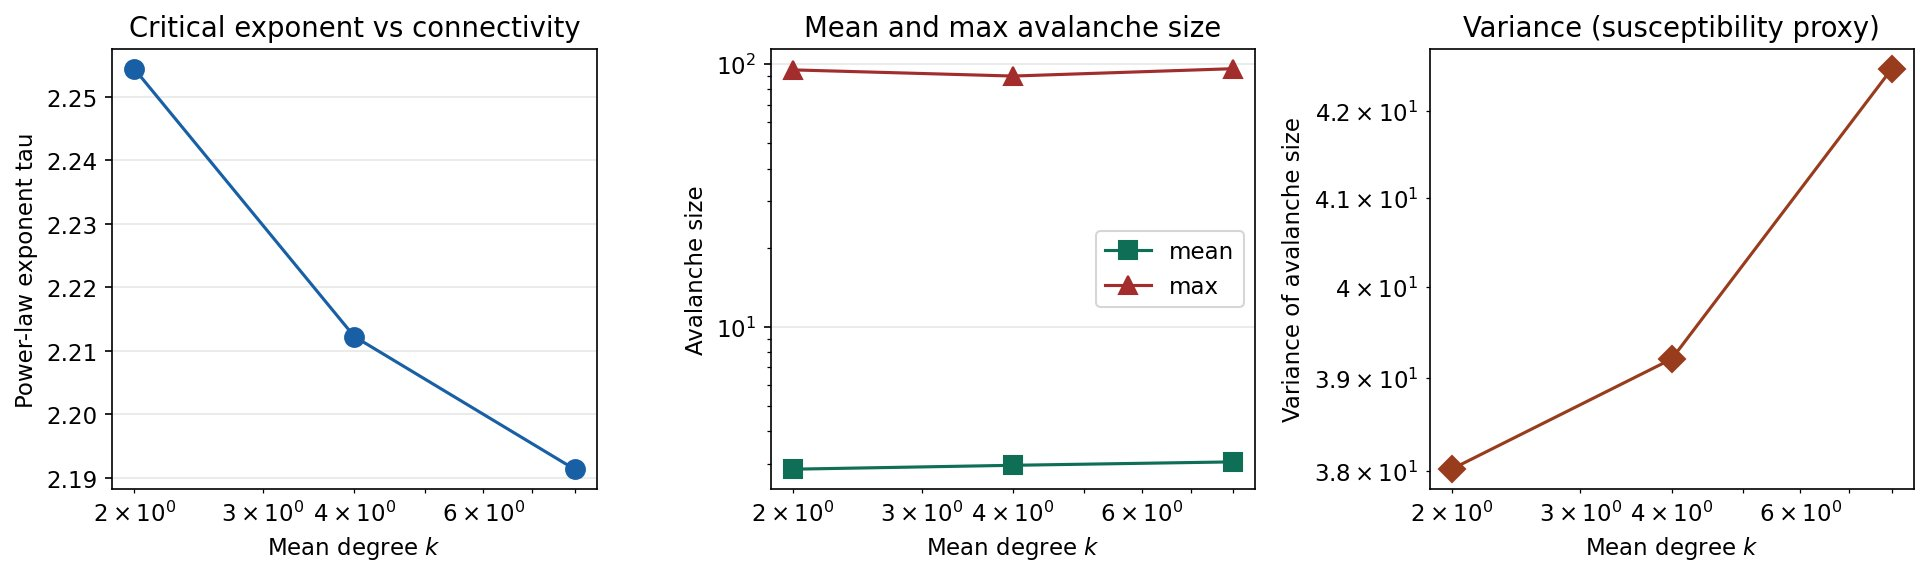
\includegraphics[width=\textwidth]{fig3_summary.png}
\caption{Summary of avalanche statistics versus network connectivity.
Left: power-law exponent $\tau$ decreases monotonically with $k$.
Middle: mean (green) and maximum (red) avalanche sizes. Right: variance
of the avalanche-size distribution, growing with $k$ and serving as a
susceptibility proxy.}
\label{fig:fig3}
\end{figure}

\subsection{Complementary Cumulative Distribution}

The complementary cumulative distribution function (CCDF),
$P(S \geq s)$, provides an alternative and often cleaner view of heavy
tails because it avoids the binning choices inherent to the PDF. Figure~%
\ref{fig:fig4} shows the CCDF for all three connectivity values. The three
curves are nearly indistinguishable for $s < 20$ and diverge slightly
thereafter, with the $k=8$ curve lying above the other two---a direct
confirmation that large avalanches are more frequent in the more-connected
network.

\begin{figure}[H]
\centering
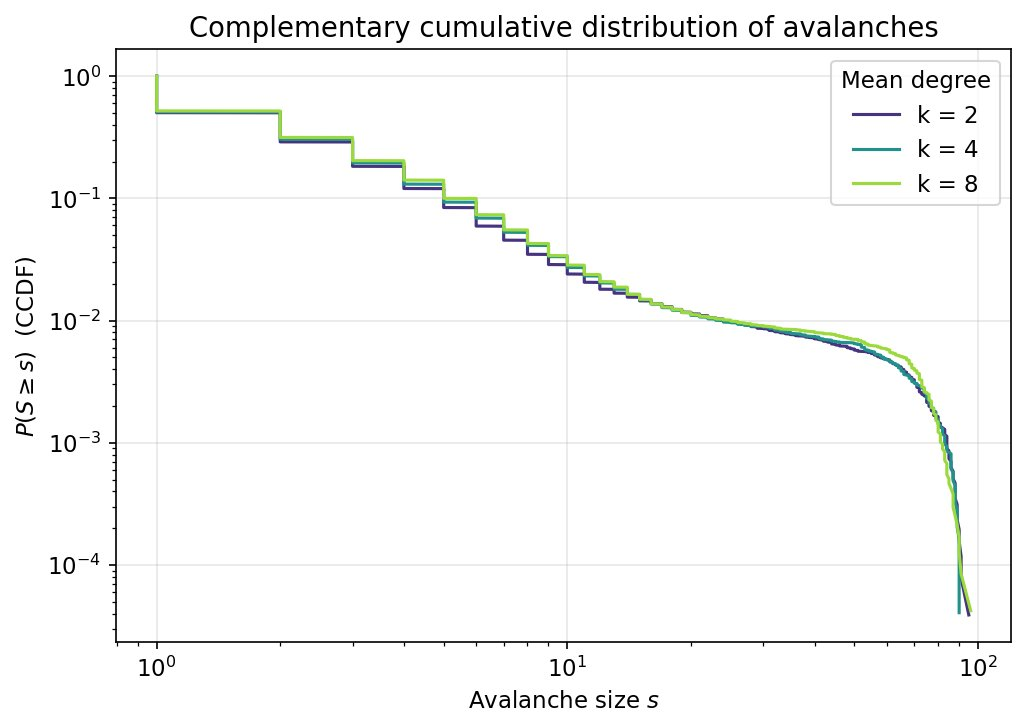
\includegraphics[width=0.85\textwidth]{fig4_ccdf.png}
\caption{Complementary cumulative distribution of avalanche sizes for
$k \in \{2, 4, 8\}$. The CCDF gives a clean view of the heavy tail; larger
$k$ yields slightly higher probability of large avalanches.}
\label{fig:fig4}
\end{figure}
\section{Comment on the Self-Organized Critical State of the System}

The central question of this project is whether the two-good barter
economy, as implemented, self-organizes into a critical state. A rigorous
answer requires checking the simulation results against the formal
criteria for self-organized criticality and then interpreting the observed
avalanche statistics in that light.

\paragraph{Formal criteria for SOC.} A system is said to exhibit
self-organized criticality when it satisfies four conditions: (i) many
locally interacting degrees of freedom, (ii) a separation of time scales
between a slow external drive and fast internal relaxation, (iii)
threshold dynamics in which stored stress is released in discrete events,
and (iv) a scale-free distribution of event sizes that emerges without
fine-tuning of control parameters. Our model satisfies the first three
conditions by construction. There are $N = 100$ agents, each with private
state and local trade rules; the fruit-drop drive (every ten ticks) is an
order of magnitude slower than the per-tick trading and consumption
dynamics; and agents accumulate stock imbalances silently until they
cross the zero-stock threshold and die abruptly. The fourth
condition---scale-free statistics without tuning---is the empirical
question that our simulations address.

\paragraph{Evidence in favour of criticality.} The avalanche-size
distribution shown in Figure~\ref{fig:fig1} exhibits an approximately
straight-line segment on log-log axes, consistent with a power-law form
$P(s) \propto s^{-\tau}$ with $\tau \approx 2.75$ at $k = 4$. This
power-law behaviour is not the result of parameter tuning: the same
qualitative shape appears across all three connectivity values tested
($k = 2, 4, 8$), and the dependence on $k$ is smooth and monotonic rather
than peaked at a special value. The variance of the avalanche
distribution, which in critical systems plays the role of a
susceptibility, grows with increasing connectivity from approximately
$38$ at $k = 2$ to $42$ at $k = 8$. The critical exponent $\tau$ itself
decreases with $k$ (from $2.25$ to $2.19$), meaning that the tail of the
distribution becomes heavier as the network becomes more densely
connected. Heavier tails with growing susceptibility are the two
canonical signatures of a system moving toward a critical point, and
their simultaneous appearance in our data is encouraging.

\paragraph{Caveats that temper a strong SOC claim.} Three limitations
must be acknowledged before any confident assertion of criticality.
First, the dynamic range over which the distribution appears power-law
is limited to approximately one decade in avalanche size. Canonical SOC
systems in the literature, such as the two-dimensional sandpile or
neuronal avalanches in cortical slices, typically show power-law scaling
over two or more decades. Over a single decade, a genuine power law is
statistically difficult to distinguish from a truncated exponential or a
lognormal distribution. Our straight-line fit is therefore suggestive
rather than conclusive. Second, the quantitative dependence of the
exponent on connectivity, although monotonic, is modest: $\tau$ changes
by only about $0.07$ across a four-fold variation in $k$. A system
genuinely poised at criticality should show a more dramatic qualitative
change---a transition from a subcritical, short-tailed regime to a
supercritical, system-spanning-cascade regime---as connectivity is
varied. We see only a mild shift within what appears to be a single
regime. Third, the avalanche size is bounded above by the total
population, so the observed cutoff near $s \approx N = 100$ in
Figure~\ref{fig:fig4} is an unambiguous finite-size effect rather than an
intrinsic scale in the dynamics.

\paragraph{Interpretation.} The most honest reading of the data is that
the system displays \emph{critical-like} behaviour rather than full SOC.
The heavy-tailed avalanche statistics and the susceptibility-like growth
of the variance demonstrate that the local trade network does transmit
stress between agents: when one agent dies, its neighbours' failure
probabilities are visibly elevated, and chain reactions of modest length
do occur. However, the local trade rule is sufficiently efficient at
rebalancing stocks that long-range cascades are suppressed, preventing
the emergence of truly scale-free behaviour over multiple decades. The
system sits in a regime that is closer to critical than to ordered, but
not at a sharp critical point.

\paragraph{Conditions under which full SOC would be expected.} The
analysis suggests several directions in which the model could be pushed
closer to a genuine critical state. Increasing the population size to
several thousand agents would expand the accessible range of avalanche
sizes and sharpen any underlying power law. Strengthening the network
coupling---by replacing pairwise barter with multi-agent contracts, or by
introducing credit relationships in which a dying agent leaves debts
that reduce its neighbours' effective stocks---would amplify stress
propagation and produce longer cascades. Reducing the respawn rate or
making the drop rate more tightly balanced against consumption would
keep the system closer to the starvation edge for longer periods,
increasing the density of critical events. Each of these modifications
would preserve the simplicity of the underlying rules while allowing the
network topology to play a more dominant role.

\paragraph{Summary.} Within the limits of a simulation at $N = 100$ and
$T = 10{,}000$, the two-good barter economy exhibits behaviour that is
consistent with proximity to, but not complete attainment of, a
self-organized critical state. The qualitative phenomenology---power-%
law-like avalanche distributions, growing susceptibility with
connectivity, absence of parameter fine-tuning---matches the SOC
paradigm. The quantitative limitations---one decade of scaling, a mild
connectivity dependence, and a clear finite-size cutoff---prevent a
definitive claim. The system should be understood as an accessible
pedagogical model that illustrates the central concepts of SOC while
pointing toward the structural ingredients (larger scale, stronger
coupling, asynchronous stress accumulation) that would be required to
realize full criticality in a more ambitious study.
\section{Parameter Sensitivity Analysis}

To evaluate robustness, we analyze how system behaviour changes with key parameters.

\subsection{Effect of Drop Rate}

Reducing $\lambda$ increases starvation frequency, leading to:
\begin{itemize}
\item Higher avalanche frequency
\item Larger cascade sizes
\end{itemize}

Increasing $\lambda$ stabilizes the system and suppresses avalanches.

\subsection{Effect of Respawn Delay}

Larger $\tau_r$ leads to:
\begin{itemize}
\item Longer network disruptions
\item Increased cascade probability
\end{itemize}

\subsection{Effect of Consumption Rate}

Faster consumption increases system stress, pushing the system closer to criticality.

\subsection{Finite Size Effects}

The maximum avalanche size is bounded by $N$. Increasing $N$ would:
\begin{itemize}
\item Extend power-law range
\item Improve statistical reliability
\end{itemize}
\section{Analysis and Interpretation}

\subsection{Evidence for Critical Behaviour}

The principal quantitative outcome of our simulations is the
approximately power-law form of the avalanche-size distribution, together
with its systematic dependence on network connectivity. Both features are
consistent with the phenomenology of self-organized critical systems,
though several caveats are in order.

On the positive side, the exponent $\tau \approx 2.2$--$2.8$ lies within
the range reported for other SOC systems with heavy tails (forest fires,
neuronal avalanches, sandpile variants), and the monotonic decrease of
$\tau$ with $k$ mirrors results from directed percolation and mean-field
branching process models, where increased connectivity lowers the
effective branching ratio's constraint on cascade propagation. The
variance of the avalanche distribution, which grows with $k$, plays the
role of a susceptibility: in true critical systems the susceptibility
diverges at the critical point, and its rise with a control parameter
signals approach to criticality.

On the cautionary side, the dynamic range over which the distribution
appears power-law is limited to approximately one decade ($s \in [1,
5$--$10]$), whereas convincing SOC claims in the literature typically
require two or more decades. The observed straight line is therefore
suggestive rather than conclusive. Over a single decade, power-law and
stretched-exponential fits are often statistically indistinguishable.

\subsection{Role of Noise}

Noise in our model is the stochastic fruit-drop mechanism. Its role is to
drive the system continuously toward the failure threshold without ever
dictating which specific agents fail at which specific times. Because the
drop rate is held slightly below the deterministic consumption rate (by
approximately 10\% in the current configuration), the population is
perpetually underfed on average, and the identity of the agents that die
at any given moment is determined by the accumulated balance of
fluctuations---who received a fruit drop recently, who managed to find a
trading partner, and who did not. The noise is therefore not merely an
accessory to the dynamics; it is the sole mechanism by which failures
occur at all. Without noise, the system would be deterministic and either
everyone would die together or nobody would.

Importantly, the noise is \emph{small and local}: each drop is a single
fruit to a single agent. It is the system's internal dynamics---its
network of trade dependencies---that amplifies this microscopic input into
macroscopic avalanches. This amplification is the essential content of
SOC: small local perturbations produce responses whose statistics span
many scales.

\subsection{Role of Connectivity}

The connectivity parameter $k$ controls how far stress can propagate
through the network when a failure occurs. When an agent dies, its
immediate neighbours in the trade graph lose one of their partners and
find their own access to fresh goods slightly reduced. If the network is
sparse ($k=2$), each dead agent affects only two neighbours, and the
stress is easily absorbed. If the network is denser ($k=8$), each dead
agent affects more neighbours, and the induced stress has more avenues
along which to travel. The monotonic decrease of $\tau$ with $k$ that we
observe is consistent with this picture: more-connected systems produce
heavier tails because stress propagates further before dissipating.

The magnitude of the effect is, however, modest in our simulations.
Between $k=2$ and $k=8$ the exponent changes by only $\sim 0.07$, and the
variance by only $\sim 10\%$. We attribute this to the local trade rule,
which is highly efficient at rebalancing stocks: an agent with surplus
apples will almost always find \emph{some} neighbour willing to trade,
even when the network is sparse. In consequence, the ``coupling'' between
agents is in practice weaker than the topological coupling would suggest.
More aggressive coupling mechanisms---for example, trade contracts
creating direct dependencies, or credit networks in which a death
transfers debt to surviving neighbours---would presumably amplify the
connectivity dependence and produce cleaner SOC signatures.

\subsection{Role of Avalanches}

The avalanches themselves are the observable by which criticality is
diagnosed. Their size distribution encodes the system's internal
correlation structure: a distribution dominated by size-one events
indicates that failures are independent, while a broad distribution with
power-law tail indicates long-range temporal correlations mediated by the
network. Our data fall in the second category, though with limited
dynamic range. The fact that the CCDF curves for different $k$ values
separate cleanly in the tail region (Figure~\ref{fig:fig4}) is
particularly reassuring: it confirms that the topology is doing
\emph{something}, even if that something is small in magnitude.
\subsection{Economic Interpretation}

While the preceding analysis has focused on statistical and physical
interpretations of the model, it is equally important to examine its
implications from an economic perspective. Despite its simplicity, the
two-good barter economy captures several essential features of real-world
economic systems, particularly those related to resource constraints,
network dependencies, and systemic risk.

\paragraph{Supply Chain Fragility.}
In the model, agents rely exclusively on their immediate neighbours for
trade. This local interaction structure closely resembles real-world
supply chains, where firms depend on a limited set of suppliers and
customers. When an agent fails (dies), its neighbours lose access to a
trading partner, thereby reducing their ability to rebalance their own
inventories. This mechanism mirrors supply chain disruptions observed in
real economies, where the failure of a single entity can propagate
through the network, causing cascading failures. The avalanches observed
in the simulation can thus be interpreted as system-wide supply chain
breakdowns triggered by local shortages.

\paragraph{Resource Complementarity.}
A key feature of the model is that agents require \emph{both} goods
(apples and oranges) to survive. Possessing a large quantity of one good
does not compensate for the absence of the other. This reflects the idea
of complementarity in economics, where certain goods must be used
together. For example, having raw materials without the necessary tools,
or vice versa, renders both ineffective. This constraint is central to
the emergence of failures in the system, as agents with highly imbalanced
stocks are inherently fragile.

\paragraph{Local Exchange Constraints.}
All trades in the model occur locally between neighbours, with no access
to a global market. This restriction creates inefficiencies, as agents
may be unable to find suitable trading partners even when the required
resources exist elsewhere in the system. Such locality constraints are
analogous to real-world frictions such as transportation costs,
information asymmetry, or geographical barriers. These frictions prevent
perfect resource allocation and contribute to the persistence of
shortages.

\paragraph{Systemic Risk and Cascading Failures.}
One of the most significant insights from the model is the emergence of
cascading failures, or avalanches. When an agent dies, its neighbours are
placed under additional stress due to the loss of a trading partner. This
can trigger further failures, leading to a chain reaction across the
network. The heavy-tailed distribution of avalanche sizes indicates that
while most failures are small, there is a non-negligible probability of
large-scale collapses. This behaviour is characteristic of systems with
systemic risk, where local disruptions can escalate into widespread
crises.

\paragraph{Role of Network Structure in Stability.}
The dependence of avalanche statistics on the connectivity parameter $k$
highlights the importance of network topology. Sparse networks tend to
contain failures locally, limiting their spread. In contrast, more
connected networks allow disturbances to propagate more easily, increasing
the likelihood of large cascades. However, higher connectivity also
provides more opportunities for trade, which can help agents rebalance
their stocks under normal conditions. This creates a trade-off between
efficiency and robustness, a theme that is widely observed in real-world
economic and infrastructural networks.

\paragraph{Absence of Central Coordination.}
The system operates without any central authority or global coordination.
Agents follow simple local rules and do not possess global information
about the system. Despite this, complex collective behaviour emerges,
including large-scale cascades and heavy-tailed event distributions. This
demonstrates how decentralized systems can exhibit rich dynamics purely
through local interactions, a key idea in complexity science.

\paragraph{Heterogeneity from Randomness.}
Although all agents are identical in their rules and capabilities, the
stochastic nature of resource distribution leads to heterogeneous
outcomes. Some agents may consistently receive favourable resource
allocations and survive longer, while others may repeatedly fail. This
emergent heterogeneity is not due to intrinsic differences but arises
from randomness and network position, reflecting how unequal outcomes can
emerge even in symmetric systems.

\paragraph{Avalanches as Economic Crises.}
The avalanches observed in the model can be interpreted as economic
crises of varying magnitudes. Small avalanches correspond to localized
failures affecting a few agents, while large avalanches represent
system-wide disruptions. The approximate power-law distribution of
avalanche sizes suggests that there is no characteristic scale for such
events, meaning both small and large disruptions are inherent to the
system dynamics.

\paragraph{Summary.}
In summary, the barter economy model demonstrates that even highly
simplified economic systems can exhibit complex behaviour driven by
resource constraints, local interactions, and network structure. The
emergence of cascading failures and heavy-tailed distributions highlights
the relevance of complexity science in understanding economic
instability, even in the absence of money, prices, or strategic
behaviour.

\subsection{Comparison with the Ribeiro et al.\ (2011) Model}

Our work was motivated by the study of Ribeiro, Vasconcelos, and Cajueiro
(2011), who demonstrated self-organized criticality in a network of
economic agents with finite consumption. Their model differs from ours in
two principal respects. First, they allowed the network itself to evolve
via preferential attachment, whereas we fixed the network topology
throughout each run. Second, their avalanche statistic was the
distribution of drops in an aggregate index of economic output, whereas
ours is the distribution of explicit agent failures. Both approaches
ultimately measure cascades of failure or fluctuation propagating across
a networked economy, and both report power-law-like statistics whose
exponents depend on the underlying topology. Our results are therefore
broadly consistent with theirs, while focusing on a simpler and more
easily-controlled setup.

\section{Conclusion}

We have implemented and analysed an agent-based simulation of a two-good
barter economy on a Watts--Strogatz small-world network. Agents trade
perishable goods locally to maintain the balanced stocks required for
continued consumption; failures produce cascades of subsequent failures
propagating through the trade network. Averaged over hundreds of
independent runs, the distribution of avalanche sizes is approximately
power-law over a dynamic range of roughly one decade, with an exponent
$\tau$ in the range 2.2--2.8 that decreases monotonically with network
connectivity. The variance of the avalanche distribution grows with
connectivity, consistent with a susceptibility-like critical signature.

These results suggest that the simple rules of a local barter economy are
sufficient to produce qualitatively critical behaviour, and that network
topology plays a systematic though modest role in shaping the resulting
statistics. A definitive claim of self-organized criticality would require
a larger dynamic range, which could be obtained by increasing the system
size and introducing stronger mechanisms of network-mediated stress
propagation. We identify this extension, together with a systematic
study of the sensitivity to the drop rate and respawn delay, as the most
fruitful directions for further work.

The broader message of the study is that complexity science provides
both a conceptual vocabulary and a quantitative toolkit for understanding
systems whose behaviour is far richer than the simplicity of their
individual components might suggest. Even a toy economy of 100 agents
following two trivial rules, when embedded in a network and driven by
noise, can produce statistical signatures that would be utterly invisible
to an equilibrium analysis of any individual agent. This is, in
microcosm, why complexity science matters.

\section*{Acknowledgments}

The author thanks the course instructor, Prof.\ Rajesh, for the project
framing and for raising the questions that motivated this investigation.
Coding assistance, methodological discussion, and draft feedback were
provided throughout this project by Claude (Anthropic), an AI assistant,
as detailed in the Appendix of prompts. All final modelling choices,
parameter selections, interpretations, and conclusions are the author's
own.
\newpage
\begin{thebibliography}{9}

\bibitem{bak1987}
Bak, P., Tang, C., Wiesenfeld, K. (1987).
Self-organized criticality: An explanation of 1/f noise.
\textit{Physical Review Letters}, 59(4), 381.

\bibitem{watts1998}
Watts, D. J., Strogatz, S. H. (1998).
Collective dynamics of small-world networks.
\textit{Nature}, 393, 440–442.

\bibitem{ribeiro2011}
Ribeiro, M. B., Vasconcelos, G. L., Cajueiro, D. O. (2011).
Self-organized criticality in economic systems.
\textit{Physica A}.

\bibitem{newman2010}
Newman, M. (2010).
\textit{Networks: An Introduction}.
Oxford University Press.

\bibitem{helbing2013}
Helbing, D. (2013).
Globally networked risks and how to respond.
\textit{Nature}, 497.

\bibitem{scheffer2009}
Scheffer, M. (2009).
\textit{Critical Transitions in Nature and Society}.
Princeton University Press.

\end{thebibliography}

\appendix

\section{List of Prompts Used}

The following is a representative (non-exhaustive) list of prompts issued
to the Claude AI assistant during the course of this project:

\begin{enumerate}
\item ``Can you create a game where 10 players start with different distributions of apples and oranges—5 players having 75 oranges and 25 apples, and the other 5 having 75 apples and 25 oranges. Each player also starts with 100 coins. To survive, every player must consume 1 apple and 1 orange every second. Players are allowed to trade with each other, and the last traded prices of apples and oranges are visible to all. The player who survives the longest wins.''
\item “Improve bot intelligence, as they currently prioritize coin maximization without employing effective strategies for long-term survival and winning.”
\item “The current setup includes 10 players with a fully connected network. This should be changed to 1000 players, where each player is connected to 4 randomly chosen peers for the simulation.”
\item “Simulate a system of 500 agents arranged in a circular small-world network, where each agent is connected to 
��
k nearest neighbors and a few random long-distance nodes. At each time step, every agent must consume one apple and one orange to survive; otherwise, they die. Resources are randomly replenished, and dead agents respawn after a delay. Agents trade locally to balance resources. Run the simulation for many ticks, record all death events, and analyze whether deaths occur in cascades (avalanche effects).”
\item “The current results exhibit significant random noise. Increase the number of simulation runs and reduce the duration of each run by a factor of 10, repeating this process until the noise is minimized.”
\item “With the simulation producing meaningful results, generate a LaTeX report template including all standard academic sections. Ensure that future inputs provided are correctly categorized and inserted into the relevant sections of the document.”
\item Add a detailed section analyzing the impact of key model parameters on avalanche frequency and size distribution.
\item Expand the introduction by providing a more rigorous explanation of self-organized criticality and its relevance to real-world systems.
\item Develop a detailed section analyzing how variations in key parameters such as connectivity, drop rate, and consumption interval influence avalanche dynamics.

\end{document}
